\documentclass{article}
\usepackage{civ}

\title{CIV102: Problem Set \#3}
\author{QiLin Xue \\ \href{mailto:qilin.xue@mail.utoronto.ca}{qilin.xue@mail.utoronto.ca} \\ TA: Michel}
\date{\today}
\usepackage{mathrsfs}
\usetikzlibrary{arrows}
\usepackage{siunitx}
\usepackage{wasysym}
\usetikzlibrary{calc}
\usepackage{xcolor}
\setlength\parindent{0pt}

\begin{document}
\maketitle
\section{Problem One: Free Vibration}
\textbf{(a)} Let us first draw a free body diagram of the person-platform system (where the person is represented by a box) at maximum tension:
\begin{center}
    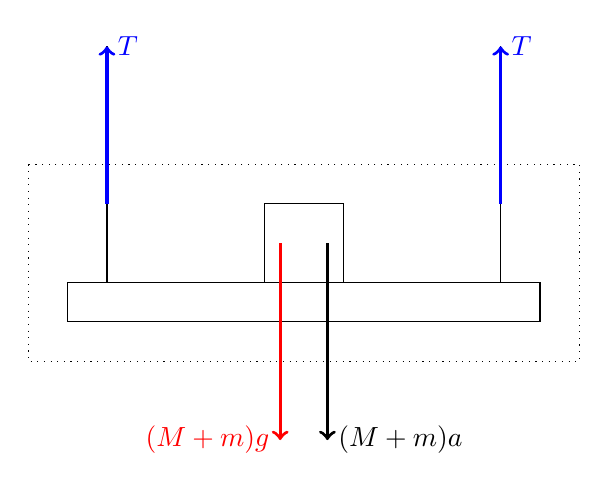
\begin{tikzpicture}
        \draw[] (-2.5,0) -- (-2.5,3);
        \draw[] (2.5,0) -- (2.5,3);
        \draw[] (-3,0) rectangle (3,-0.5);
        \draw[] (-0.5,0) rectangle (0.5,1);
        \draw[dotted] (-3.5,1.5) rectangle (3.5,-1);
        \draw[color=blue,very thick,->] (-2.5,1) -- (-2.5,3) node[right] {$T$};
        \draw[color=blue,very thick,->] (2.5,1) -- (2.5,3) node[right] {$T$};
        \draw[color=red,very thick,->] (-0.3,0.5) -- (-0.3,-2) node[left] {$(M+m)g$};
        \draw[color=black,very thick,->] (0.3,0.5) -- (0.3,-2) node[right] {$(M+m)a$};
    \end{tikzpicture}
\end{center}
where we have applied D'alembert's principle at the maximum elongation. Thus, the system is in equilibrium and balancing forces in the vertical direction gives:
\begin{equation}
    2T=(M+m)g+(M+m)a
    \label{eq:d'alambert-platform}
\end{equation}
where $m$ is the mass of the person and $M$ is the mass of the platform. We can also draw the free body diagram of the person:
\begin{center}
    \begin{tikzpicture}
        \draw[] (-2.5,0) -- (-2.5,3);
        \draw[] (2.5,0) -- (2.5,3);
        \draw[] (-3,0) rectangle (3,-0.5);
        \draw[] (-0.5,0) rectangle (0.5,1);
        \draw[color=red,very thick,->] (0,0.5) -- (-0,3) node[left] {$F$};
        \draw[color=black,very thick,->] (0.3,0.5) -- (0.3,-1.5) node[right] {$ma$};
        \draw[color=red,very thick,->] (-0.3,0.5) -- (-0.3,-1.5) node[left] {$mg$};
    \end{tikzpicture}
\end{center}
Balancing forces yet again gives:
\begin{equation}
    mg+ma=F
    \label{eq:d'alambert block}
\end{equation}
where $F$ is the force from the ground. Solving for $F$ and then substituting it into equation (\ref{eq:d'alambert-platform}) gives:
\begin{equation}
    2T=(M+m)g+(M+m)\frac{F-mg}{m} \implies F = \frac{m}{M+m}(2T)
    \label{eq:}
\end{equation}
The tension force can be calculated using Hooke's Law:
\begin{equation}
    T = EA\epsilon = 3927\si{\newton}
    \label{eq:alambert-tension}
\end{equation}
where $E=10,000\si{\mega\pascal}$ is the Young's Modulus, $A=\frac{\pi d^2}{4}$ is the cross sectional area of the rope with diameter $d=10\si{\milli\meter}$, and the strain is $\epsilon=\frac{15}{3000}$. Using this tension force, we get:
\begin{equation}
    \boxed{F=3140\si{\newton}}
    \label{eq:}
\end{equation}
\textbf{(b)} First, we can calculate the spring constant of each rope to be:
\begin{equation}
    k = \frac{EA}{L_0} = 261,799 \si{\newton\per\meter}
    \label{eq:}
\end{equation}
Then the total energy stored in both ropes is:
\begin{equation}
    W = 2 \cdot \underbrace{\left(\frac{1}{2}k\Delta L^2\right)}_\text{energy of each} = \boxed{58.9\si{\joule}}
    \label{eq:}
\end{equation}
We can determine the stress in each rope to be:
\begin{equation}
    \sigma = E\epsilon = 50\si{\mega\pascal}
    \label{eq:}
\end{equation}
and thus the safety factor as:
\begin{equation}
    f = \frac{\sigma_\text{ult}}{\sigma} = \boxed{1.200}.
    \label{eq:}
\end{equation}
While it won't break in an ideal world, this might not be the best design!

\textbf{(c)} We can treat the two ropes as one rope just as long but with double the area. Since the spring constant $k=EA/L$ scales linearly with area, the effective spring constant is:
\begin{equation}
    k_\text{eff} = 2k
    \label{eq:}
\end{equation}
We can then plug this into the formula for natural frequency to get:
\begin{equation}
    f = \frac{1}{2\pi}\sqrt{\frac{2k}{m+M}} = \boxed{8.14\si{\hertz}}.
    \label{eq:}
\end{equation}
\newpage
\section{Problem Two: Poisson's Ratio}
\textbf{(a)} High tensile steel has a yield strength of $\sigma_\text{yield}=1650\si{\mega\pascal}$ and a Young's Modulus of $E=200,000\si{\mega\pascal}$. The longitudinal strain $\epsilon_x$ needed is given by:
\begin{equation}
    \sigma_\text{yield} = E\epsilon_x \implies \epsilon_x = \frac{\sigma_\text{yield}}{E} = \boxed{8.25 \times 10^{-3}}
    \label{eq:}
\end{equation}
This gives the radial strain as $\epsilon_y=\epsilon_z = -\mu \epsilon_l$. And thus the area changes by a factor of:
\begin{equation}
    \frac{\Delta A}{A} = \epsilon_y\epsilon_z = \mu^2 \epsilon_x^2
    \label{eq:}
\end{equation}
Note that $\Delta A$ denotes a decrease in area and the original area is $A=9\si{\milli\meter\squared}$. The force associated with this is:
\begin{equation}
    F = \sigma_\text{yield}(A-\Delta A)=\sigma_\text{yield}A(1-\mu^2\epsilon_x^2)=\boxed{14,850\si{\newton}}
    \label{eq:}
\end{equation}
Note that the factor of $1-\mu^2\epsilon_x^2$ is so small, it doesn't affect the final answer (after rounding to four sig digs).

\textbf{(b)} Using the definition for Poisson's ratio, we can determine the transverse strain as:
\begin{equation}
    \epsilon_y=\epsilon_z=-\mu \epsilon_x=\boxed{2.48 \times 10^{-3}}
    \label{eq:}
\end{equation}
The change in volume is then:
\begin{equation}
    \frac{\Delta V}{V} = \frac{\Delta(xyz)}{xyz}=(1+\epsilon_x)(1+\epsilon_y)(1+\epsilon_y)-1 = (1+\epsilon_x)(1-0.3\epsilon_x)^2 - 1
    \label{eq:}
\end{equation}
so the change in volume is:
\begin{equation}
    \Delta V= xyz \frac{\Delta V}{V} =\boxed{46.9\si{\milli\meter\cubed}}
    \label{eq:}
\end{equation}
\textbf{(c)} We want $\frac{\Delta V}{V}=0$, or:
\begin{equation}
    (1+\epsilon_x)(1-\mu \epsilon_x)^2=1
    \label{eq:}
\end{equation}
Solving for $\mu$ gives:
\begin{equation}
    \mu = \frac{1-\sqrt{\frac{1}{1+\epsilon_x}}}{\epsilon_x}
    \label{eq:}
\end{equation}
Substituting in $\epsilon_x$, we get: $\boxed{\mu=0.497}.$ This seems pretty close to $\mu=0.5$ and indeed, if the strain is small enough it will always hover around this region. We can do this by taking the limit as $\epsilon_x \to 0$. Since this is not ESC194, I hope I can get away with a non-rigorous way of doing this by taking the first order binomial expansion:
\begin{equation}
    \mu = \frac{1-(1+\epsilon_x)^{-1/2}}{\epsilon_x}\approx \frac{1-(1-\frac{1}{2}\epsilon_x)}{\epsilon_x}=\frac{1}{2}
    \label{eq:}
\end{equation}
Intuitively, this comes from the fact (which comes from error analysis, which in turn comes from the derivative of a square) that:
\begin{equation}
    \frac{\Delta A}{A} = 2\frac{\Delta r}{r}
    \label{eq:}
\end{equation}
where $r=y=z$ is the width.

\newpage
\section{Problem Three}
Let's first draw a good diagram with well chosen variables:
\begin{center}
    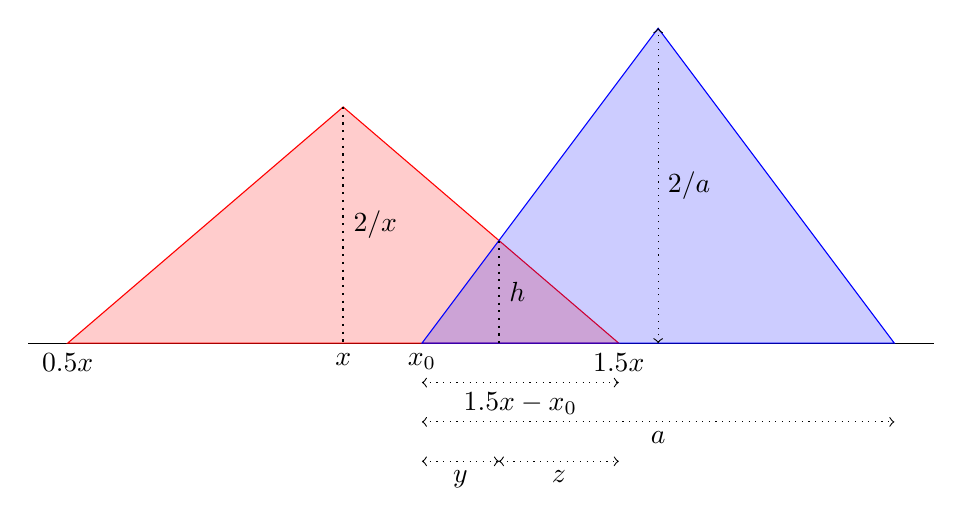
\begin{tikzpicture}
        \draw[] (0,0) -- (11.5,0);
        \draw[fill=red,draw=red,fill opacity=0.2] (0.5,0) -- (4,3) -- (7.5,0) -- cycle;
        \draw[fill=blue,draw=blue,fill opacity=0.2] (5,0) -- (8,4) -- (11,0) -- cycle;
        \draw[thick,dotted] (4,3) -- (4,0) node[midway,right] {$2/x$};
        \draw[thick,dotted] (5.978,1.304) -- (5.978,0) node[midway,right] {$h$};
        \draw[thick] (4,0) node[below] {$x$};
        \draw[thick] (5,0) node[below] {$x_0$};
        \draw[thick] (7.5,0) node[below] {$1.5x$};
        \draw[thick] (0.5,0) node[below] {$0.5x$};

        \draw[<->,dotted] (5,-0.5) -- (7.5,-0.5) node[midway,below] {$1.5x-x_0$};
        \draw[<->,dotted] (5,-1.5) -- (5.978,-1.5) node[midway,below] {$y$};
        \draw[<->,dotted] (5.978,-1.5) -- (7.5,-1.5) node[midway,below] {$z$};

        \draw[<->,dotted] (5,-1) -- (11,-1) node[midway,below] {$a$};
        \draw[<->,dotted] (8,0) -- (8,4) node[midway,right] {$2/a$};
    \end{tikzpicture}
\end{center}
We want the area of the shaded region to equal $f=0.02$ and the dimensions are picked such that the areas are normalized (e.g. equal to one). We have three equations:
\begin{align}
    y+z&=1.5x-x_0 \label{eq:y+z} \\ 
    \frac{y}{h}&=\frac{a^2}{4} \label{eq:y/h} \\ 
    \frac{z}{h}&=\frac{x^2}{4} \label{eq:z/h}
\end{align}
where the last two equations comes from similar triangles, by breaking the middle triangle into two right angled ones, then comparing the side lengths of each half with the red triangle and the blue triangle. Using equation (\ref{eq:y+z}), we can rewrite (\ref{eq:y/h}) as:
\begin{equation}
    \frac{1.5x-x_0-z}{h}=\frac{a^2}{4}
    \label{eq:}
\end{equation}
and combining it with equation (\ref{eq:z/h}) gives:
\begin{equation}
    1.5x-x_0-\frac{hx^2}{4}=\frac{ha^2}{4} \implies h = \frac{1.5x-x_0}{x^2/4+a^2/4}
    \label{eq:}
\end{equation}
We demand that the area of the triangle be equal to $f=0.02$:
\begin{equation}
    A = \frac{1}{2}(1.5x-x_0)h = f \implies \frac{1}{2}(1.5x-x_0)\frac{1.5x-x_0}{x^2/4+a^2/4}=f
    \label{eq:}
\end{equation}
which we can solve:
\begin{align}
    (1.5x-x_0)^2&=\frac{f}{2}(x^2+a^2)\\
    4.5x^2-6xx_0+2x_0^2 &=fx^2+fa^2\\ 
    (4.5-f)x^2+(-6x_0)x+(2x_0^2-fa^2) &= 0 \\
    4.48x^2-9720x+5246208&= 0
\end{align}
and using the quadratic equation gives us:
\begin{equation}
    \sigma_\text{allow} \equiv 1008\si{\mega\pascal}, 1161 \si{\mega\pascal}
    \label{eq:}
\end{equation}
The first solution is not physical, since $1.5\sigma_\text{allow}$ doesn't even cross into the blue triangle region. Therefore, the answer is $\boxed{\sigma_\text{allow}=1161\si{\mega\pascal}}$ and the factor of safety is:
\begin{equation}
    \text{FOS} = \frac{1800}{1161}=1.550.
    \label{eq:}
\end{equation}
\newpage
\section{Problem Four}
\textbf{(a)} Here, we essentially have two rods in series and we can no longer assume that each rod has the same strain. However, the two rods will have the same force, which we can use to calculate the stress:
\begin{equation}
    F_\text{max}=\sigma_1A_1=\sigma_2A_2 \implies \sigma_1d_1^2=\sigma_2d_2^2
    \label{eq:}
\end{equation}
 where $A_1>A_2$. As a result, $\sigma_1 < \sigma_2 = \sigma_\text{yield}$. Similarly, we can then calculate the strain in each part of the nonuniform rod:
\begin{equation}
    E\epsilon_1A_1=E\epsilon_2A_2
    \label{eq:}
\end{equation}
We can summarize the results:
\begin{align}
    \sigma_2 &= \sigma_\text{yield} \\
    \sigma_1 &= \sigma_\text{yield}\left(\frac{d_2}{d_1}\right)^2 \\ 
    \epsilon_2 &= \frac{\sigma_\text{yield}}{E} \\ 
    \epsilon_1 &= \frac{\sigma_\text{yield}}{E}\left(\frac{d_2}{d_1}\right)^2
\end{align}
so the elastic energy stored in the rope is given by:
\begin{equation}
    W = \frac{V_1}{2}\frac{\sigma_\text{yield}^2}{E}\left(\frac{d_2}{d_1}\right)^4+\frac{V_2}{2}\frac{\sigma_\text{yield}^2}{E}
    \label{eq:}
\end{equation}
which simplifies to:
\begin{equation}
    W = \frac{\pi L}{8}\frac{\sigma_\text{yield}^2}{E}\left(d_1^2\left(\frac{d_2}{d_1}\right)^4+d_2^2\right)
    \label{eq:}
\end{equation}
The total change in length is:
\begin{equation}
    \Delta L = L(\epsilon_1+\epsilon_2)=\frac{L\sigma_\text{yield}}{E}\left(1+\left(\frac{d_2}{d_1}\right)^2\right)
    \label{eq:}
\end{equation}
Conservation of energy gives:
\begin{equation}
    mg(h+\Delta L)=W \implies h = \frac{1}{mg}\frac{\pi L}{8}\frac{\sigma_\text{yield}^2}{E}\left(d_1^2\left(\frac{d_2}{d_1}\right)^4+d_2^2\right)-\frac{L\sigma_\text{yield}}{E}\left(1+\left(\frac{d_2}{d_1}\right)^2\right)=\boxed{0.360\si{\meter}}
    \label{eq:cons}
\end{equation}

\textbf{(b)} If dropping the weight higher than part (a), we will start to see plastic deformation. Since the two wires are made of the same material, and have the same tension but different areas, the thinner (bottom) wire will experience a larger stress. By Hooke's Law $\sigma = \sigma \epsilon$, the bottom wire will experience a larger strain as well. Since the strain of the bottom wire is larger than the top, it would experience yielding first.
\vspace{2mm}

While the bottom wire is yielding, the strain increases without changing the stress and thus the force is unchanged. This implies two things. First, the top wire stays static since its stress is also unchanged. Because the force experienced by the weight is constant, it will follow a parabolic path.
\vspace{2mm}

Once the weight stops at the bottom of its parabolic trajectory, the bottom wire will deform according to Hooke's Law. But because the bottom wire has elongated beforehand, it does not go back to its original length. We are in fact able to calculate just how much this change of length is. Suppose the weight is dropped from a height $H=h+\Delta h$ where $h$ is as determined above. Then there would be some leftover kinetic energy $\frac{1}{2}mv^2=mg\Delta h$ once the bottom wire starts experiencing yielding. Conservation of energy gives:
\begin{equation}
    mg(\Delta h+\Delta L_\text{extra}) =F\Delta L_\text{extra} = \underbrace{\frac{EA}{L}\Delta L}_\text{constant}(\Delta L_\text{extra}) \implies \Delta h = 364\Delta L
    \label{eq:}
\end{equation}
We won't analyze in much detail, but after the yielding, the stress will start increasing again until the upper wire starts yielding and a similar thing occurs: The tension force remains constant, so the bottom wire will maintain the same length while the upper wire elongates.

\textbf{(c)} This problem got me at first... It may be tempting to say that in the new case (with one long thin wire) will break first because it cannot store as much energy as before so for a given height, the strain needs to be longer to compensate for it, thus reaching its maximum elongation faster.
\vspace{2mm}

This reasoning is false because it doesn't mention how the energy is distributed. For example, perhaps the majority of the energy in the old case could be concentrated in the thin wire. Since the old thin wire has a smaller volume than the new thin wire, it will break first. This in reality, is exactly what happens and we are going to prove it.
\vspace{2mm}

First and perhaps the easiest proof is by directly plugging $d_1=6\si{\milli\meter}$ in equation (\ref{eq:cons}) to give a maximum height of $0.631\si{\milli\meter}$. As a result, the new setup can withstand a drop from nearly twice as high and still be in the elastic region! This equation still applies because we can model one long wire as two identical wires half as long. That equation can be a bit long so it might not be obvious why this number increased, but it becomes more clear if we look at two springs in series with spring constants $k_1$ and $k_2$ such that:
\begin{equation}
    W=\frac{1}{2}k_1x_1^2+\frac{1}{2}k_2x_2^2
    \label{eq:}
\end{equation}
and
\begin{equation}
    k_1x_1=k_2x_2
    \label{eq:}
\end{equation}
which we can combine to get:
\begin{equation}
    W = \frac{1}{2}k_2x_2^2\left(1+\frac{k_2}{k_1}\right)
    \label{eq:}
\end{equation}
As the spring constant of the upper wire $k_1$ increases, the factor $1+k_2/k_1$ increases. And for a given energy $W$, this means the displacement $x_2$ decreases. (If you want to view this in terms of strain, you can let $k_2=EA/L$ and let the strain to be $x_2/L$, which still decreases.)
\vspace{2mm}

Second, it is also helpful to look at an extreme case where the area of the top half is huge, say on the order of magnitude of the ceiling of a room. Then hopefully intuitively one can see that practically speaking, it's possible to completely ignore the energy stored in the top wire. For a similar reason when doing my pendulum lab for physics, I don't analyze the strain caused by my tiny mass on the roof, even if I used something elastic for my string!
\vspace{2mm}

I will show why the above is true quantitatively and rigorously by looking at the effective spring constant. Consider two springs with spring constants of $k_1$ and $k_2$ connected in series where spring one is fixed at one end.Suppose the free end of the first spring displaces by $\Delta x_1$ and the other end of spring $2$ displaces by $\Delta x_2$ relative to the contact point. Since the tension is constant throughout, we must have
    \begin{equation}
        k_1\Delta x_1=k_2\Delta x_2
        \label{eq:}
    \end{equation}
    We want to find the effective spring constant $k_\text{eff}$ such that the force can also be written as:
    \begin{equation}
        k_2\Delta x_2=k_\text{eff}(\Delta x_1+\Delta x_2)
        \label{eq:}
    \end{equation}
    Making the substitution $\Delta x_1=\frac{k_2}{k_1}\Delta x_2$, we can cancel out factors of $\Delta x_2$ to get:
    \begin{equation}
        k_2=k_\text{eff}\left(\frac{k_2}{k_1}+1\right) \implies k_\text{eff} = \frac{k_1k_2}{k_1+k_2}
        \label{eq:}
    \end{equation}
    Taking the approximation where $k_1 \ll k_2$, we get:
    \begin{equation}
        k_\text{eff}=k_2
        \label{eq:}
    \end{equation}
For the nonuniform wire, the effective spring constant is very nearly equal to the spring constant of the bottom wire. Therefore, the old system behaves as if there was only a $1$ meter long wire while the new system behaves as a $2$ meter long wire. Therefore for a given strain, the new case can extend about twice as long as the old case, hence explaining the rough factor of $2$ we saw earlier.
\vspace{2mm}

One final thing for intuition: Recall that the effective spring constant equation resembles finding the effective resistance of two resistors in parallel. Since a circuit analogy might be more intuitive for others, I have included this bonus. A circuit and a system of springs actually have a lot in common. Here are the analogies one can make:
\begin{align}
    \text{spring constant}  &\iff \text{resistance} \\
    \text{displacement}     &\iff \text{current} \\ 
    \text{potential energy} &\iff \text{electrical power} 
    \label{eq:}
\end{align}
There are others involving inductors and capacitors, but these are the relevant ones for now. As a result, this question is exactly equivalent to this: Consider an appliance made of two resistors $R$ and $r$ connected in parallel, and needs a total power of $P$ to run. We want to minimize the current going through resistor $r$. Would letting $R \gg r$ or $R=r$ be a better choice? If $R \gg r$, then the majority of the current will flow through the branch with resistor $r$. Since we want to minimize this flow, then it makes sense for $R=r$. This completely agrees with the argument earlier that the one long thin wire will last longer.
% Thus, the effective spring constant for this setup is:
% \begin{equation}
%     k_\text{eff} = 4.958\si{\mega\newton\per\meter}
%     \label{eq:}
% \end{equation}
% where I have plugged in $E=200000\si{\mega\pascal}$, $L=1\si{\meter}$, and the relevant diameters $d_1=16\si{\milli\meter}$ and $d_2=6\si{\milli\meter}$ into:
% \begin{equation}
%     k_i=\frac{E\pi d_i^2}{4L}
%     \label{eq:}
% \end{equation}
% for each of $i\in \{1,2\}$. The yield strength of low alloy steel is $\sigma_\text{yield}=420\si{\mega\pascal}$, leading to a maximum change in length of:
% \begin{equation}
%     \sigma_\text{yield} = E\frac{\Delta L}{L} \implies \Delta L = \frac{\sigma_\text{yield}L}{E} = 0.0021\si{\meter}
%     \label{eq:}
% \end{equation}
% From conservation of energy, we must have:
% \begin{equation}
%     mg(h+\Delta L)=\frac{1}{2}k(\Delta L)^2 \implies h_\text{max}=\frac{\frac{1}{2}k_\text{eff}(\Delta L)^2-mg\Delta L}{mg}=\boxed{0.276\si{\meter}}
%     \label{eq:}
% \end{equation}
% where $m=4\si{\kilogram}$ and $g=9.81\si{\meter\per\second\squared}$.
\end{document}
